\batchmode
\makeatletter
\def\input@path{{"C:/Users/tkpme/Dropbox/BookPCRA/Springer Production March 2026/Ch Appendix C Utility Theory/"}}
\makeatother
\documentclass[graybox,envcountchap,sectrefs]{svmono}\usepackage[]{graphicx}\usepackage[]{xcolor}
% maxwidth is the original width if it is less than linewidth
% otherwise use linewidth (to make sure the graphics do not exceed the margin)
\makeatletter
\def\maxwidth{ %
  \ifdim\Gin@nat@width>\linewidth
    \linewidth
  \else
    \Gin@nat@width
  \fi
}
\makeatother

\definecolor{fgcolor}{rgb}{0.345, 0.345, 0.345}
\newcommand{\hlnum}[1]{\textcolor[rgb]{0.686,0.059,0.569}{#1}}%
\newcommand{\hlsng}[1]{\textcolor[rgb]{0.192,0.494,0.8}{#1}}%
\newcommand{\hlcom}[1]{\textcolor[rgb]{0.678,0.584,0.686}{\textit{#1}}}%
\newcommand{\hlopt}[1]{\textcolor[rgb]{0,0,0}{#1}}%
\newcommand{\hldef}[1]{\textcolor[rgb]{0.345,0.345,0.345}{#1}}%
\newcommand{\hlkwa}[1]{\textcolor[rgb]{0.161,0.373,0.58}{\textbf{#1}}}%
\newcommand{\hlkwb}[1]{\textcolor[rgb]{0.69,0.353,0.396}{#1}}%
\newcommand{\hlkwc}[1]{\textcolor[rgb]{0.333,0.667,0.333}{#1}}%
\newcommand{\hlkwd}[1]{\textcolor[rgb]{0.737,0.353,0.396}{\textbf{#1}}}%
\let\hlipl\hlkwb

\usepackage{framed}
\makeatletter
\newenvironment{kframe}{%
 \def\at@end@of@kframe{}%
 \ifinner\ifhmode%
  \def\at@end@of@kframe{\end{minipage}}%
  \begin{minipage}{\columnwidth}%
 \fi\fi%
 \def\FrameCommand##1{\hskip\@totalleftmargin \hskip-\fboxsep
 \colorbox{shadecolor}{##1}\hskip-\fboxsep
     % There is no \\@totalrightmargin, so:
     \hskip-\linewidth \hskip-\@totalleftmargin \hskip\columnwidth}%
 \MakeFramed {\advance\hsize-\width
   \@totalleftmargin\z@ \linewidth\hsize
   \@setminipage}}%
 {\par\unskip\endMakeFramed%
 \at@end@of@kframe}
\makeatother

\definecolor{shadecolor}{rgb}{.97, .97, .97}
\definecolor{messagecolor}{rgb}{0, 0, 0}
\definecolor{warningcolor}{rgb}{1, 0, 1}
\definecolor{errorcolor}{rgb}{1, 0, 0}
\newenvironment{knitrout}{}{} % an empty environment to be redefined in TeX

\usepackage{alltt}
\usepackage{mathptmx}
\usepackage{helvet}
\usepackage{courier}
\usepackage[T1]{fontenc}
\usepackage[utf8]{inputenc}
\usepackage{geometry}
\geometry{verbose,tmargin=1in,bmargin=1in,lmargin=1in,rmargin=1in}
\setcounter{tocdepth}{3}
\setlength{\parskip}{\medskipamount}
\setlength{\parindent}{0pt}
\usepackage{float}
\usepackage{units}
\usepackage{textcomp}
\usepackage{amsmath}
\usepackage{amssymb}
\usepackage{graphicx}
\PassOptionsToPackage{normalem}{ulem}
\usepackage{ulem}
\usepackage[unicode=true,pdfusetitle,
 bookmarks=true,bookmarksnumbered=true,bookmarksopen=true,bookmarksopenlevel=1,
 breaklinks=false,pdfborder={0 0 1},backref=false,colorlinks=false]
 {hyperref}
\hypersetup{
 pdfstartview=XYZ null null 1.25,pdfpagemode=UseNone}

\makeatletter
%%%%%%%%%%%%%%%%%%%%%%%%%%%%%% User specified LaTeX commands.
%%%%%%%%%%%%%%%%%%%% book.tex %%%%%%%%%%%%%%%%%%%%%%%%%%%%%
%
% sample root file for the chapters of your "monograph"
%
% Use this file as a template for your own input.
%
%%%%%%%%%%%%%%%% Springer-Verlag %%%%%%%%%%%%%%%%%%%%%%%%%%


% RECOMMENDED %%%%%%%%%%%%%%%%%%%%%%%%%%%%%%%%%%%%%%%%%%%%%%%%%%%


% choose options for [] as required from the list
% in the Reference Guide

\usepackage{makeidx}% allows index generation
% standard LaTeX graphics tool
                             % when including figure files
\usepackage{multicol}% used for the two-column index
\usepackage[bottom]{footmisc}% places footnotes at page bottom

\usepackage{hyperref}
\def\UrlBreaks{\do\/\do-}

% see the list of further useful packages
% in the Reference Guide

\makeindex             % used for the subject index
                       % please use the style svind.ist with
                       % your makeindex program


%\usepackage[ style=authoryear,natbib=true,giveninits=true,backend=biber,maxcitenames=2]{biblatex}
\usepackage[style=authoryear,natbib=true,firstinits=false,backend=biber,maxcitenames=2]{biblatex}


\setlength{\bibitemsep}{0.5\baselineskip}
\DeclareNameAlias{sortname}{family-given}

\IfFileExists{C:/Users/Doug/Dropbox/BookPCRA/mpslbookCombined.bib}
{\addbibresource[location=local]{C:/Users/Doug/Dropbox/BookPCRA/mpslbookCombined.bib}}
{   \IfFileExists{C:/Users/tkpme/Dropbox/BookPCRA/mpslbookCombined.bib}
    {\addbibresource[location=local]{C:/Users/tkpme/Dropbox/BookPCRA/mpslbookCombined.bib}}
    {   \IfFileExists{C:/Users/stoya/Dropbox/BookPCRA/mpslbookCombined.bib}
        {\addbibresource[location=local]{C:/Users/stoya/Dropbox/BookPCRA/mpslbookCombined.bib}}
        {   \IfFileExists{C:/Users/4thauthor/Dropbox/BookPCRA/mpslbookCombined.bib}
            {\addbibresource[location=local]{C:/Users/4thauthor/Dropbox/BookPCRA/mpslbookCombined.bib}}
            {}
        }
    }
}
\renewcommand\cite{\citet}

\usepackage{amsmath}
\usepackage{amssymb}
\usepackage[p,osf]{stickstootext}
\usepackage[stix2,vvarbb]{newtxmath}
\usepackage[varqu,varl]{inconsolata}
% \usepackage{txfonts}
\usepackage{upgreek}

\DeclareMathOperator{\argmax}{arg\,max}
\DeclareMathOperator{\argmin}{arg\,min}
\usepackage{array}
\usepackage{arydshln}
\usepackage{booktabs}
\usepackage{threeparttablex}
\usepackage{appendix}

\usepackage[utf8]{inputenc}
%%%%%%%%%%%%%%%%%%%%%%%%%%%%%%%%%%%%%%%%%%%
\IfFileExists{C:/Users/Doug/Dropbox/BookPCRA/macroSP_August_05_2021.tex}
{\input{C:/Users/Doug/Dropbox/BookPCRA/macroSP_August_05_2021.tex}}
{   \IfFileExists{C:/Users/tkpme/Dropbox/BookPCRA/macroSP_August_05_2021.tex}
    {\input{C:/Users/tkpme/Dropbox/BookPCRA/macroSP_August_05_2021.tex}}
    {   \IfFileExists{C:/Users/stoya/Dropbox/BookPCRA/macroSP_August_05_2021.tex}
        {\input{C:/Users/stoya/Dropbox/BookPCRA/macroSP_August_05_2021.tex}}
        {   \IfFileExists{C:/Users/4thAuthor/Dropbox/BookPCRA/macroSP_August_05_2021.tex}
            {\input{C:/Users/4thAuthor/Dropbox/BookPCRA/macroSP_August_05_2021.tex}}
            {}
        }
    }
}

\belowsink=90pt


%%%%%%%%%%%%%%%%%%%%%%%%%%%%%%%%%%%%%%%%%%%%%

\makeatother
\IfFileExists{upquote.sty}{\usepackage{upquote}}{}
\begin{document}
\begin{appendices}


\setcounter{chapter}{2} 

\chapter{UTILITY THEORY\label{chap:AppendixC}}

\vspace{0.3in}

\textbf{Planned for publication in 2026 by R. Douglas Martin, Thomas
K. Philips, Bernd Scherer and Kirk Li. All rights reserved. © Copyright
2025}

\vspace{0.3in}

\begin{center}
10/12/25
\par\end{center}

\tocchpnum=30pt 
\tocsecnum=33pt 
\tocsubsecnum=40pt 
\tocsubsubsecnum=48pt 
\tocparanum=55pt 
\tocsubparanum=63pt
\calctocindent

\tableofcontents{}\newpage{}

\section{Investor Preferences and Utility Functions \label{sec: investorPreferencesConcaveUtilityFncs}}

The question of how to choose among investment opportunities (or,
more generally, among uncertain prospects) has a rich history, with
interdisciplinary contributions by gamblers, economists, mathematicians
and psychologists\footnote{Mathematicians and gamblers worked more closely than one might imagine
-- mathematicians often derived results and sold them to gamblers
for immediate use in the field!}. Early on, it was broadly accepted that the fair price of entry to
a game of chance was the expected value of its payoff. By way of example,
if the flip of a coin returned \$0 or \$2 with equal probability,
the fair price for participation in this game was held to be $0.5\cdot\$0+0.5\cdot\$2=\$1$.
But in 1710, Nicolaus Bernoulli described a simple game, now known
as the St. Petersburg game, that threw this belief into doubt. The
St. Petersburg game is played as follows: 

A fair coin is repeatedly flipped, and the number of flips till the
first appearance of a head, which we denote by $k$, is noted. The
gambler is then paid $\$2^{k}$ for participating in the game. As
the probability of first seeing a head on the $k^{th}$ flip is $\nicefrac{1}{2^{k}}$,
the expected payoff from this game is

\begin{align}
E\left[\mathrm{Payoff}\right] & =\sum_{k\,\geqslant\,1}\frac{1}{2^{k}}\cdot\$2^{k}\nonumber \\
 & =\infty.\label{eq:StPetersburgPayoff}
\end{align}

But no gambler would pay an infinite amount to participate in this
game. In practice, gamblers seem to be willing to pay no more than
about \$20 for the privilege of participating in the St. Petersburg
game, a paradox if there ever was one! 

Nicolas Bernoulli's cousin Daniel\footnote{The Bernoullis were a remarkable family, as well known for their contributions
to mathematics as for their feuds.} attempted to resolve the paradox by positing that the pleaure (or
\emph{utility}) associated with a \$1 increase in wealth would be
the reciprocal of the initial level of wealth, and that gamblers could
therefore be expected to have logarithmic utility for wealth\footnote{As we shall see, these two views are mathematically equivalent. In
modern language, Daniel Bernoulli asserted that the marginal utility
of wealth was the reciprocal of wealth.}. The expected utility from participating in the St. Petersburg game
is therefore

\begin{align}
E\left[\ln\left(\mathrm{Payoff}\right)\right] & =\sum_{k\,\geqslant\,1}\frac{1}{2^{k}}\cdot\ln\left(2^{k}\right)\nonumber \\
 & =\sum_{k\,\geqslant\,1}\frac{k}{2^{k}}\cdot\ln\left(2\right)\nonumber \\
 & =2\ln\left(2\right),\label{eq:StPetersburgUtility}
\end{align}

which is finite.

\citet{Moscati2019} traces the evolution of resolutions to this paradox,
and also exposes the vigorous debates between competing schools of
thought that finally settled down in the decade following the publication
of an axiomatic theory of utility by John von Neumann and Oskar Morgenstern
(VNM) in 1947. The VNM axioms are expressed in terms of preferences
over random outcomes (or ``lotteries''). We write $X\succ Y$ to
express a strong preference for lottery $X$ over lottery $Y$, and
$X\sim Y$ to express indifference between the two lotteries. Likewise,
we write $X\succeq Y$ to express a weak preference for lottery $X$
over lottery $Y$. By definition, 

\begin{equation}
X\succeq Y\equiv X\succ Y\ \mathrm{or}\ X\sim Y.\label{eq:XWeaklyPreferredToY}
\end{equation}

\begin{description}
\item [{\textbf{Axiom}}] \textbf{1 (Completeness)}: All lotteries can be
ranked. For any pair of lotteries $X$ and $Y$, either $X\succ Y$,
or $Y\succ X$, or $X\sim Y$.
\item [{\textbf{Axiom}}] \textbf{2 (Transitivity)}: For any three lotteries
$X,\ Y$ and $Z$, if $X\succeq Y$ and $Y\succeq Z$, then $X\succeq Z$.
\item [{\textbf{Axiom}}] \textbf{3 (Substitution)}: For any three lotteries
$X,\ Y$ and $Z$, if $X\succeq Y\succeq Z$, then $Y\sim p\,X+(1-p)\,Z$
for some $p\in[0,1]$, where $p\,X+(1-p)\,Z$ is interpreted as participation
in lottery $X$ with probability $p$ and participation in lottery
$Z$ with probability $1-p$.
\end{description}
\citet{VonNeumann1947} proved that if investors' preferences satisfied
these three axioms, they would choose among risky alternatives so
as to maximize their expected utility, and in spite of many fits,
starts, and paradoxes, \emph{Expected Utility Maximization} (EUM)
has come to be the dominant paradigm for modeling choice in economics\footnote{Some authors use a more fine-grained set of axioms, see for example
the discussions of utility theory in \citet{Levy2016}}. 

EUM requires investors to express their preferences via a \emph{cardinal
utility function}\footnote{Cardinal utility assign a real number to each outcome of interest.
Ordinal utility, in contrast, only specifies if one outcome is preferred
to another.} $U(\mathit{\mathrm{v}})$ that is a dimensionless function of investment
end--of--period wealth $\mathit{\mathrm{v}}$, and which is invariant
under an affine transformation, $\check{U}(\mathit{\mathrm{v}})=a+b\cdot\mathit{U}(\mathit{\mathrm{v}}),\ b>0$,
in the sense that $\check{U}$ and $U(\mathit{\mathrm{v}})$ provide
the same ranking among investment alternatives. 

Suppose an investor's preferences can be captured by such a utility
function, whose values are sometimes referred to as \emph{utils},
and she chooses an investment that maximizes expected end--of--period
utility $\mathrm{E}\left[U(\mathrm{V})\right]$. The form of the utility
function $U$ will depend on the assumptions one makes about her preferences,
and we next determine the implications of two simple and reasonable
assumptions concerning investor preferences for utility functions:
\begin{description}
\item [{P1:}] \textbf{Non-satiation}: At any level of wealth $\mathrm{v}_{1}$,
the investor prefers a strictly larger wealth $\mathrm{v}_{2}>\mathrm{v}_{1}$.
\item [{P2:}] \textbf{Risk Aversion}: The investor maximizes her expected
utility, and is\emph{ risk averse} in the following sense: she always
prefers a fixed end of period wealth, $\mathrm{v}_{0}$, to a \emph{fair
game} in which end of period wealth is the random amount $\mathrm{V}=\mathrm{v}_{0}+\text{H}$\footnote{This is one of those occasions where it is useful to represent a random
variable with a capital letter to distinguish it from an variable
that is non--random (such as a particular realization) and so represented
by a lower case letter.}, where $\mathrm{H}$ has mean zero and variance $\sigma^{2}>0$.
\end{description}
We note in passing that investors are said to \emph{weakly risk averse
}if they are indifferent to participating in such a fair game.\footnote{Much of the utility theory literature uses the term ``strictly risk
averse'' where we use ``risk averse'', and uses ``risk averse''
where we use ``weakly risk averse''.} 

These assumptions are not all--encompassing -- the near--universal
existence of casinos and lotteries indicates that there is no shortage
of individuals who prefer (or sadly, are addicted to) the expected
losses and uncertain outcomes that are endemic to gambling. Even more
interesting, risk--averse and risk--seeking behavior can co-exist
in the same individual: a great many people buy both life insurance
and lottery tickets!

An investor with preferences P1 and P2 will use a utility function
with the following properties:
\begin{description}
\item [{U1.}] $U(\mathit{\mathrm{v}})$ is strictly increasing in $\mathit{\mathrm{v}}$,
\item [{U2.}] $U(\mathit{\mathrm{v}})$ is strictly concave\footnote{A \emph{strictly concave} function is one for which a straight line
connecting two distinct points on the $U(\mathit{\mathrm{v}})$ curve
lies strictly below the curve, except at the two end-points where
the line joins the curve, as in the left--hand plot in Figure \ref{fig: ShapesOfUtilityFunctions}.
The mathematical definitions of concave and concave functions are
given in Appendix A.}.
\end{description}
The utility property U1 follows immediately from P1. The concavity
property U2 follows from P2 and Jensen's inequality\footnote{See the discussion of convex and concave functions, as well as of
Jensen's inequality, in Appendix A}. 

\begin{figure}[H]
\begin{centering}
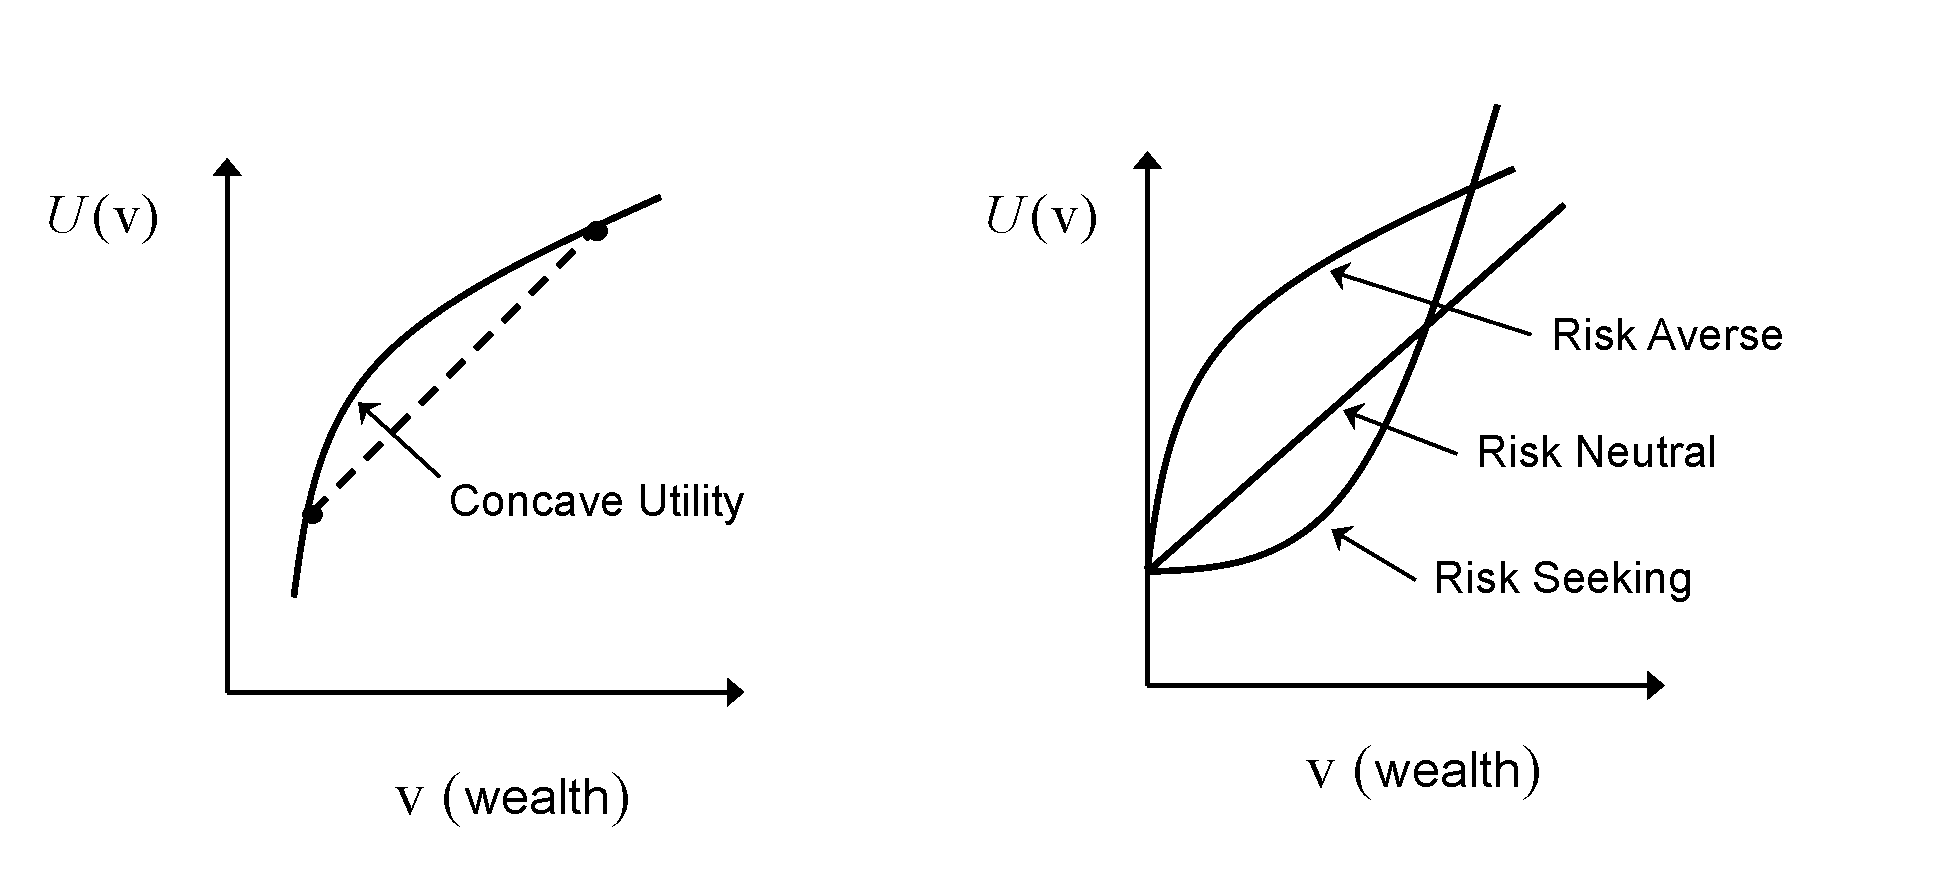
\includegraphics[scale=0.5]{2C__Users_tkpme_Dropbox_BookPCRA_Springer_Produ___ity_Theory_Plots_concave_utility_risk_prefs.png}
\par\end{centering}
\caption{Shapes of Utility Functions}

\label{fig: ShapesOfUtilityFunctions}
\end{figure}

The commonly occurring utility functions described in the next subsection
have both first and second derivatives, and for such utility functions
the properties U1 and U2 are equivalent to the following derivative
properties:
\begin{description}
\item [{U1E:}] $U^{\prime}(\mathit{\mathrm{v}})>0$
\item [{U2E:}] $U^{\prime\prime}(\mathit{\mathrm{v}})<0$
\end{description}
The first derivative of $U$ is known as its \emph{marginal utility},
and represents the increase in utility obtained from an additional
dollar of wealth. While a\emph{ }risk averse EUM investor is one whose
differentiable utility function is concave, a \emph{risk seeking}
EUM investor is one whose utility function is strictly convex\emph{}\footnote{A \emph{strictly convex} utility function is one that satisfies the
U2E property with the inequality sign reversed. }\emph{.} An investor with a utility function that has a constant first
derivative, and hence a zero second derivative, is said to be \emph{risk
neutral}. 

\section{Concave Utility Functions and Risk Aversion}

With property P2 in mind, consider the fair investment game with end-of-period
wealth $\mathrm{V}=\mathrm{v}_{0}+\mathrm{H}$, where

\begin{equation}
\mathrm{H}=\left\{ \begin{array}{cl}
\,\,\,\mathrm{h}_{1}:\ -\mathrm{v}_{0}<\mathrm{h}_{1}<0, & \mbox{with probability \ensuremath{p}}\\
\mathrm{h}_{2}:\ 0<\mathrm{h}_{2},\ \ \ \ \ \ \ \ \ \, & \mbox{with probability \ensuremath{1-p}}
\end{array}\right.\label{eq: fairGame}
\end{equation}

with any fixed $\mathrm{h}_{1}$ and $\mathrm{h}_{2}$ such that

\begin{equation}
\mathrm{E}\left[\mathrm{H}\right]=p\,\mathrm{h}_{1}+(1-p)\,\mathrm{h}_{2}=0,\label{eq:E_H_eq_0}
\end{equation}

so that $\mathrm{E}\left[\mathrm{V}\right]=\mathrm{v}_{0}$. 

For this fair game, we have

\begin{equation}
\mathrm{E}\left[U\left(\mathrm{V}\right)\right]=p\cdot U\left(\mathrm{v}_{0}+\mathrm{h}_{1}\right)+\left(1-p\right)\cdot U\left(\mathrm{v}_{0}+\mathrm{h}_{2}\right),\label{eq:E_U_of_V}
\end{equation}

and since $U(\mathrm{v}_{0})=\mathrm{E}\left[U(\mathrm{v}_{0})\right]$,
we also have:

\begin{equation}
\mathrm{E}\left[U(\mathrm{v}_{0})\right]=U\left(p\cdot\left(\mathrm{v}_{0}+\mathrm{h}_{1}\right)+\left(1-p\right)\cdot\left(\mathrm{v}_{0}+\mathrm{h}_{2}\right)\right).\label{eq:E_U_of_V_0}
\end{equation}

Since by P2 our EUM investor is risk averse, she prefers the sure
outcome $\mathrm{v}_{0}$ to the risky outcome $\mathrm{V}$, and
as she is also an expected utility maximizer, it must be that $\mathrm{E}\left[U(\mathrm{v}_{0})\right]>\mathrm{E}\left[U(\mathrm{V})\right]$,
and accordingly we have

\begin{equation}
U\left(p\cdot\left(\mathrm{v}_{0}+\mathrm{h}_{1}\right)+\left(1-p\right)\cdot\left(\mathrm{v}_{0}+\mathrm{h}_{2}\right)\right)>p\cdot U\left(\mathrm{v}_{0}+\mathrm{h}_{1}\right)+\left(1-p\right)\cdot U\left(\mathrm{v}_{0}+\mathrm{h}_{2}\right)\label{eq:E_U_V_0_gt_U_E_V_0}
\end{equation}

for all combinations of $\mathrm{v}_{0},\ -\mathrm{v}_{0}<\mathrm{h}_{1}<0$,
and $0<\mathrm{h}_{2}$ that satisfy \eqref{eq:E_H_eq_0}, which is
the same as asserting that

\begin{equation}
U\left(p\cdot\mathrm{v}_{1}+(1-p)\cdot\mathrm{v}_{2}\right)>p\cdot U\left(\mathrm{v}_{1}\right)+(1-p)\cdot U\left(\mathrm{v}_{2}\right),\ \forall\,\mathrm{v_{1}}<\mathrm{v}_{2}.\label{eq: strictConcavityCondition}
\end{equation}

But the above inequality is equivalent to the statement that $U$
is a strictly concave function. 

\section{Certainty Equivalent Value and the Risk Premium}

Sometimes portfolio managers want to compare portfolios that have
different expected utilities in terms of monetary units rather the
dimensionless units of utility functions. One way in which to do so
is to define a dollar amount, $\mathit{\mathrm{v}}_{c}$, known as
the \emph{Certainty Equivalent Value}, that satisfies the equation: 

\begin{align}
U(\mathit{\mathrm{v}}_{c}) & =\mathrm{E}[U(\mathrm{V})]\nonumber \\
 & \implies\mathit{\mathrm{v}}_{c}=U^{-1}\left(\mathrm{E}[U(\mathrm{V})]\right).\label{eq: certaintyEquivalent}
\end{align}

We interpret $\mathit{\mathrm{v}}_{c}$ as the lower, sure, value
that a risk--averse investor would accept in place of the risky payoff
$\mathrm{V}$, with higher expected value $\mathrm{E}\left[\mathrm{V}\right]$,
in order to avoid the uncertainty associated with the random character
of $\mathrm{V}$. Figure \ref{fig: certaintyEquivValue} shows graphically
how such a value is obtained for a risk--averse investor when end--of--period
random wealth $\mathrm{V}$ has expected utility $\mathrm{E}\left[U(\mathrm{V})\right]$.
Note that $\mathit{\mathrm{v}}_{c}$ is less than $\mathrm{E}\left[\mathrm{V}\right]$,
in accordance with Jensen's equality for a (strictly) concave function,
which asserts that $\mathrm{E}\left[U(\mathrm{V})\right]<U\left(\mathrm{E}\left[\mathrm{V}\right]\right)$
(see Appendix A). Thus
\[
U(\mathrm{v}_{c})=\mathrm{E}\left[U(\mathrm{V})\right]<U\left(\mathrm{E}\left[\mathrm{V}\right]\right)
\]

and since $U$ is strictly increasing, it follows that $\mathrm{v}_{c}<\mathrm{E}[\mathrm{V}]$.

\begin{figure}[H]
\begin{centering}
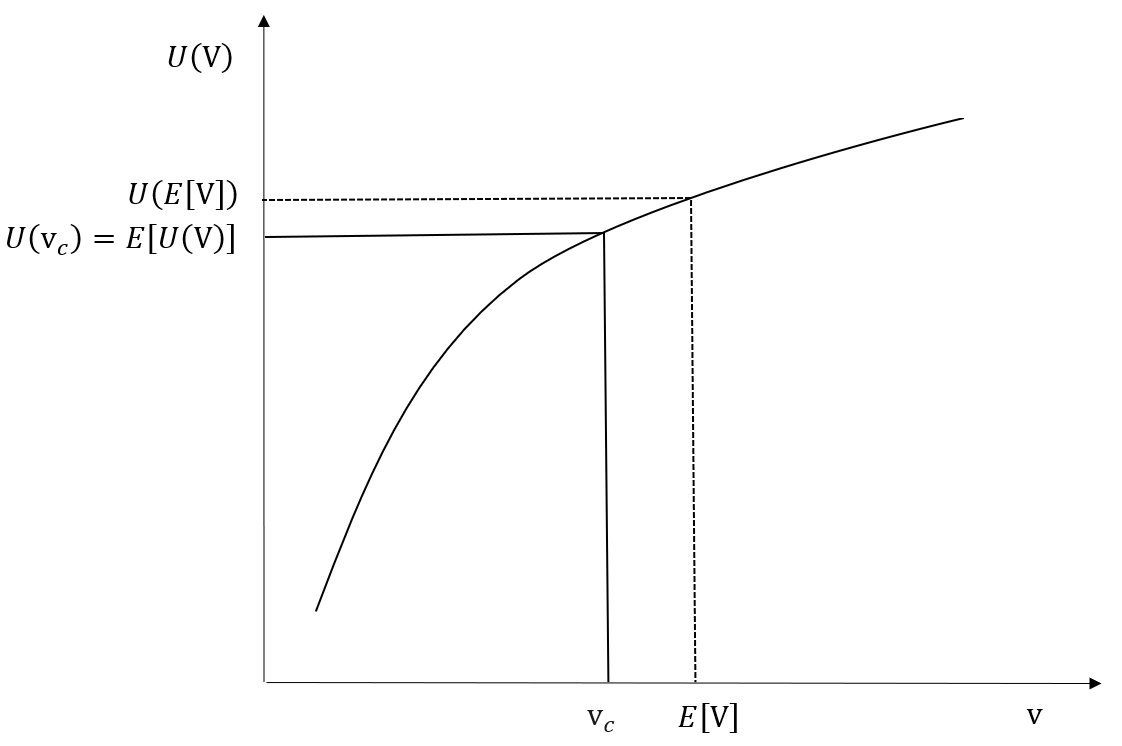
\includegraphics[scale=0.3]{3C__Users_tkpme_Dropbox_BookPCRA_Springer_Produ____C_Utility_Theory_Plots_certaintyEquivalent.png}
\par\end{centering}
\caption{Certainty Equivalent Value for Expected Utility}

\label{fig: certaintyEquivValue}
\end{figure}

 Correspondingly, the \emph{Absolute Risk Premium}, $\pi_{A}\left(\mathrm{v}\right)$
is 

\begin{equation}
\pi_{A}\left(\mathrm{E}\left[\mathrm{V}\right]\right)=\mathrm{E}\left[\mathrm{V}\right]-\mathit{\mathrm{v}}_{c},\label{eq:AbsoluteRiskPremium}
\end{equation}

and this can be interpreted as the amount of wealth the investor is
willing to forego (or the insurance premium she is willing to pay)
to avoid the risk of a fair investment game. It can also be interpreted
as the payment she would require in order to induce her to participate
in a fair game.

Closely related to the Absolute Risk Premium is the \emph{Relative
Risk Premium}, or the fraction of her wealth that a risk averse investor
would pay to avoid the risk of a fair investment game (or would have
to be paid in order to induce her to participate in a fair investment
game):

\begin{align}
\pi_{R}\left(\mathrm{E}\left[\mathrm{V}\right]\right) & =\frac{\pi_{A}\left(\mathrm{E}\left[\mathrm{V}\right]\right)}{\mathrm{E}\left[\mathrm{V}\right]}\nonumber \\
 & =\frac{\mathrm{E}\left[\mathrm{V}\right]-\mathit{\mathrm{v}}_{c}}{\mathrm{E}\left[\mathrm{V}\right]}.\label{eq:RelativeRiskPremium}
\end{align}


\section{Absolute and Relative Risk Aversion\label{sec: derivationOfRiskAversionFncs}}

The risk premium is a function both of how uncertain an investment
is and the shape of the investor's utility curve, and we so separate
the contributions of these two influences. Once again, let $\mathrm{v}_{0}$
be an initial level of wealth, let $\mathrm{V}=\mathrm{v}_{0}+\mathrm{H}$
with random payoff $\mathrm{H}$ be the end-of-period random wealth,
and let $U({\rm V})$ be the investor's utility function. Suppose
further that the investment is a fair game with $\mathrm{E}\left[\mathrm{H}\right]=0$,
and let $\sigma_{{\rm V}}^{2}$ be the variance of ${\rm H}.$ Let
$\mathrm{v}_{c}$ be the certainty equivalent for $\mathrm{E}\left[{\rm V}\right]$
and $\pi_{A}\left(\mathrm{V}\right)$ be the associated absolute risk
premium. 

If we expand $U(\mathrm{V})$ in a two--term Taylor series around
its mean, we get

\begin{align}
U(\mathrm{V}) & \thickapprox U(\mathrm{\mathit{\mathrm{E}}\left[\mathrm{V}\right]})\,+\,U^{\prime}(\mathrm{\mathit{\mathrm{E}}\left[\mathrm{V}\right]})\left(\mathrm{V}-\mathrm{\mathit{\mathrm{E}}\left[\mathrm{V}\right]}\right)\,+\,\frac{1}{2}\cdot U^{\prime\prime}(\mathrm{V})\left(\mathrm{V}-\mathrm{\mathit{\mathrm{E}}\left[\mathrm{V}\right]}\right)^{2}\nonumber \\
 & =U(\mathrm{v}_{0})\,+\,U^{\prime}(\mathrm{\mathrm{v}_{0}})\left(\mathrm{V}-\mathrm{\mathrm{v}_{0}}\right)\,+\,\frac{1}{2}\cdot U^{\prime\prime}(\mathrm{v}_{0})\left(\mathrm{V}-\mathrm{\mathrm{v}_{0}}\right)^{2}\label{eq:UtilityTaylorSeries1}
\end{align}

where the second line follows from the observation that $\mathrm{E}\left[\mathrm{V}\right]=\mathrm{v}_{0}+\mathrm{E}\left[\mathrm{H}\right]=\mathrm{v}_{0}$. 

Likewise, we can perform a one-term Taylor series expansion of $U(\mathrm{V})$
around its mean and write

\begin{align}
U(\mathrm{\mathit{\mathrm{v}}_{c}}) & \thickapprox U(\mathrm{\mathit{\mathrm{E}}\left[\mathrm{V}\right]})\,+\,U^{\prime}(\mathrm{\mathit{\mathrm{E}}\left[\mathrm{V}\right]})\left(\mathrm{\mathit{\mathrm{v}}_{c}}-\mathrm{\mathit{\mathrm{E}}\left[\mathrm{V}\right]}\right)\nonumber \\
 & =U(\mathrm{v}_{0})\,+\,U^{\prime}(\mathrm{\mathrm{v}_{0}})\left(\mathrm{\mathit{\mathrm{v}}_{c}}-\mathrm{\mathrm{v}_{0}}\right).\label{eq:UtilityTaylorSeries2}
\end{align}

On taking the expectation of both sides of \eqref{eq:UtilityTaylorSeries1},
we see that

\begin{align}
\mathrm{E}\left[U(\mathrm{V})\right] & \triangleq U(\mathrm{v}_{c})\nonumber \\
 & \thickapprox U(\mathrm{v}_{0})\,+\,\frac{1}{2}\cdot U^{\prime\prime}(\mathrm{v}_{0})\cdot\sigma_{H}^{2}\label{eq:UtilityTaylorSeries3}
\end{align}

Equating \eqref{eq:UtilityTaylorSeries2} and \eqref{eq:UtilityTaylorSeries3}
and simplifying, we get

\begin{align}
\mathrm{\mathit{\mathrm{v}}_{0}}-\mathrm{\mathrm{v}_{c}} & \triangleq\pi_{A}\left(\mathrm{\mathit{\mathrm{v}}_{0}}\right)\nonumber \\
 & =-\frac{1}{2}\cdot\frac{U^{\prime\prime}(\mathrm{v}_{0})}{U^{\prime}(\mathrm{v}_{0})}\cdot\sigma_{H}^{2}\nonumber \\
 & =\frac{1}{2}\cdot\mathrm{\mathit{ARA}(\mathrm{v}_{0})}\cdot\sigma_{H}^{2},\label{eq:UtilityTaylorSeries5}
\end{align}

where Absolute Risk Aversion is defined to be 

\begin{equation}
\mathrm{\mathit{ARA}(\mathit{\mathrm{v}})}=-\frac{\mathrm{\mathit{U}''(\mathrm{v})}}{\mathrm{\mathit{U}'(\mathit{\mathrm{v}})}}.\label{eq: ARAfunction}
\end{equation}

We can derive a similar expression for Relative Risk Aversion starting
with \eqref{eq:RelativeRiskPremium}:

\begin{align}
\pi_{R}\left(\mathrm{v}_{0}\right) & =\frac{\pi_{A}\left(\mathrm{v}_{0}\right)}{\mathrm{v}_{0}}\nonumber \\
 & =-\frac{1}{2}\cdot\frac{U^{\prime\prime}(\mathrm{v}_{0})}{U^{\prime}(\mathrm{v}_{0})}\cdot\frac{\mathrm{v}_{0}}{\mathrm{v}_{0}^{2}}\cdot\sigma_{H}^{2}\nonumber \\
 & =-\frac{1}{2}\cdot\frac{U^{\prime\prime}(\mathrm{v}_{0})\cdot\mathrm{v}_{0}}{U^{\prime}(\mathrm{v}_{0})}\cdot\sigma_{\nicefrac{H}{\mathrm{v}_{0}}}^{2}\nonumber \\
 & =\frac{1}{2}\cdot\mathrm{\mathit{RRA}(\mathrm{v}_{0})\cdot\sigma_{\nicefrac{H}{\mathrm{v}_{0}}}^{2}}\label{eq:UtilityTaylorSeries6}
\end{align}

where Relative Risk Aversion (RRA) is defined as:

\begin{align}
\mathrm{\mathit{RRA}(\mathit{\mathrm{v}})} & =\mathrm{v}\cdot ARA(\mathit{\mathrm{v}})\nonumber \\
 & =-\frac{\mathrm{v}\cdot\mathrm{\mathit{U}^{\prime\prime}(\mathrm{v})}}{\mathrm{\mathit{U}^{\prime}(\mathit{\mathrm{v}})}}.\label{eq:RRAFunction}
\end{align}

Given the relationship between ARA and RRA functions in \eqref{eq:RRAFunction},
it is clear that a constant relative risk aversion (CRRA) investor
must exhibit decreasing ARA.

Both ARA and RRA characterize utility functions locally, but it is
their global behavior for all possible values of $\mathrm{v}$ that
makes them useful in practice. Empirical evidence suggests that most
investors exhibit decreasing absolute risk aversion (i.e. they are
more willing to risk a fixed amount of money as their wealth increases),
but Relative Risk Aversion is known to depend in a complex way on
age, sex, and wealth, among other characteristics (see \citet{BellanteGreen2004}
and \citet{HalekEisenhauer2001} for good discussions of this important
point). It is therefore common practice to simply assume that investors
exhibit Constant Relative Risk Aversion (i.e. to assume that the fraction
of their wealth that they are willing to risk is independent of its
level). 

\subsection*{}

\subsection*{Marginal Utility and Risk Aversion of Common Utility Functions}

We next explore the marginal utility, as well as the absolute and
relative risk aversions, of some common utility functions. As risk
aversion is rooted both in human psychology and in our environment\footnote{Investors often become more risk seeking in good times (such as the
run up to the Internet bubble in the late 1990s) and more risk averse
in bad times (such as the period immediately following the start of
the Great Financial Crisis in 2008).}, it is not easy to divine the true shape of an investor's utility
function or degree of risk aversion. It has therefore become common
practice to focus attention on utility functions that are analytically
tractable, or which correspond to easily visualized economic goals.

\medskip{}

\uline{Logarithmic (or Log) Utility}

For log utility

\begin{equation}
\mathit{U}(\mathit{\mathrm{v}})=\ln(\mathrm{v}),\ \mathrm{v}>0,\label{eq:LogUtility}
\end{equation}

so that $\mathit{U^{\prime}}(\mathit{\mathrm{v}})=\nicefrac{1}{\mathrm{v}}$
and $\mathit{U^{\prime\prime}}(\mathit{\mathrm{v}})=-\nicefrac{1}{\mathrm{v}^{2}}$
for positive $\mathrm{v}$, and from \eqref{eq: ARAfunction} and
\eqref{eq:RRAFunction} we get:

\begin{subequations}
\begin{align}
ARA\left(\mathrm{v}\right) & =\frac{1}{\mathrm{v}},\label{eq:ARALogUtility}\\
RRA\left(\mathrm{v}\right) & =1.\label{eq:RRALogUtility}
\end{align}
\end{subequations}

The marginal utility of wealth, $\mathit{U^{\prime}}(\mathit{\mathrm{v}})$,
is $\nicefrac{1}{\mathrm{v}}$, just as Daniel Bernoulli posited.
Logarithmic utility plays an important role in finance, as it is closely
related to the geometric mean, and we explore the link between the
two in Section \ref{sec:MakingUtiliyTheoryPractical}.

\medskip{}

\uline{Generalized Logarithmic (or GLUM) Utility}

Generalized logarithmic utility is an exceptionally powerful and underappreciated
variant of log utility. It was introduced in \citet{Rubinstein1976}
and \citet{Rubinstein1977} as a flexible alternative to the CAPM,
but did not achieve widespread popularity. It allows for a wide range
of investor preferences, and lends itself naturally to the management
of assets and liabilities, as both are easily interpreted as terms
in the utility function. Formally

\begin{equation}
\mathit{U}(\mathit{\mathrm{v}})=\ln(\mathrm{v}+A),\ \mathrm{v}>-A,\label{eq:GLUMUtility}
\end{equation}

so that $\mathit{U^{\prime}}(\mathit{\mathrm{v}})=\nicefrac{1}{\left(\mathit{\mathrm{v}}+A\right)}$
and $\mathit{U^{\prime\prime}}(\mathit{\mathrm{v}})=-\nicefrac{1}{\left(\mathit{\mathrm{v}}+A\right)^{2}}$
for $\mathrm{v}>-A$, and from \eqref{eq: ARAfunction} and \eqref{eq:RRAFunction}
we get:

\begin{subequations}
\begin{align}
ARA\left(\mathrm{v}\right) & =\frac{1}{\mathrm{v}+A},\label{eq:ARAGLUMUtility}\\
RRA\left(\mathrm{v}\right) & =\frac{\mathrm{v}}{\mathrm{v}+A}.\label{eq:RRAGLUMUtility}
\end{align}
\end{subequations}

The marginal utility of wealth, $\mathit{U^{\prime}}(\mathit{\mathrm{v}})$,
is clearly decreasing in wealth, as is Absolute Risk Aversion. More
importantly, Relative Risk Aversion is increasing, constant, or decreasing
in wealth according to whether $A$ is positive, zero, or negative,
allowing a wide range of investor preferences to be parsimoniously
modeled. If we interpret $-A$ as the present value of the investor's
liabilities, $\mathrm{v}+A$ is her \emph{actuarial surplus}, or \emph{discretionary
wealth}: she could, in principle at least, lose all of it, and still
be able to meet her spending commitments. This is equivalent to the
requirement that $\mathrm{v}+A>0$.The Generalized Logarithmic Utility
function is therefore of great importance when modeling the wealth
of households, and of insurers, who have large portfolios of assets
that are offset by similar large portfolios of liabilities.

Generalized logarithmic utility is sometimes expressed in terms of
returns as

\begin{equation}
\mathit{U}(r)=\frac{\ln(1+\lambda\,r)}{\lambda},\ r>-\frac{1}{\lambda},\ \lambda>0,\label{eq:GLUMreturn}
\end{equation}

and expanding \eqref{eq:GLUMreturn} in a two-term Taylor series around
$r=0$ gives

\begin{equation}
U(r)\approx r\,-\,\frac{\lambda}{2}r^{2}.\label{eq:GLUMexpansion}
\end{equation}
Taking expecations on both sides of \eqref{eq:GLUMreturn} gives

\begin{align}
E\left[U(r)\right] & \approx E\left[r\right]\,-\,\frac{\lambda}{2}\left(\sigma^{2}\,+\,E\left[r\right]^{2}\right)\nonumber \\
 & \approx E\left[r\right]\,-\,\frac{\lambda}{2}\,\sigma^{2}\label{eq:GLUMexpansion2}
\end{align}

which closely mimics the form of the Quadratic Utility function described
in \MVOSection, allowing us to identify $\lambda$ as a measure of
risk aversion. 

\citet{WilcoxZieffSatchell2025} use \eqref{eq:GLUMreturn} and \eqref{eq:GLUMexpansion2}
to allow the identification of $\lambda$ by asking an investor a
single question: ``What is $f_{max}$, the largest fraction of your
\emph{financial} wealth you can lose without it ruining your life?''
Viewed through the lens of \eqref{eq:GLUMreturn}, this is equivalent
to identifying the most negative return $r_{max}=-f_{max}$ that the
investor can tolerate; at this return, her financial wealth is reduced
to 0 and her utility becomes infinitely negative. 

\citet{WilcoxZieffSatchell2025} argue that it proves effective in
practice to set $\lambda=\nicefrac{1}{f_{max}}$. If the investor
can lose all her financial wealth, $\lambda=1$, and she will invest
log-optimally. Many investors say that they can lose between one-quarter
and one-half of their financial wealth, corresponding to values of
$\lambda$ between 2 and 4, which corresponds remarkably well to the
range of $\lambda$ obtained through the use of more complex and comprehensive
questionnaires.

\medskip{}

\uline{Power Utility}

A power utility function has the form

\begin{equation}
\mathrm{\mathsf{\mathit{U}}(v;\,\gamma)}=\dfrac{\mathrm{v}^{1-\gamma}}{1-\gamma},\quad\mathrm{v}>0,\quad\gamma>0,\quad\gamma\neq1\label{eq:PowerUtility}
\end{equation}

It is an easy exercise to show that power utility has the risk aversion
functions:

\begin{subequations}
\begin{align}
ARA\left(\mathrm{v}\right) & =\frac{\gamma}{\mathit{\mathrm{\mathrm{v}}}},\label{eq:ARAPowerUtility}\\
RRA\left(\mathrm{v}\right) & =\gamma.\label{eq:RRAPowerUtility}
\end{align}
\end{subequations}

and marginal utility

\begin{equation}
\mathit{U^{\prime}}(\mathit{\mathrm{v}})=\mathrm{v}^{-\gamma}.\label{eq:MarginalPowerUtility}
\end{equation}

As $\gamma\longrightarrow1$, power utility converges to logarithmic
utility, and this is easily seen by applying L'Hospital's rule to
\eqref{eq:PowerUtility}. Investors who are attracted to the CRRA
and long run growth properties of logarithmic utility, but who find
it too risky for their taste, will find that power utility offers
much of what logarithmic utility does, but with the ability to control
risk by making an appropriate choice for $\gamma$.

\medskip{}

\uline{Exponential Utility}

The exponential utility function has the form

\begin{equation}
U(\mathrm{v})=\frac{1-\mathrm{exp}(-c\cdot\mathrm{v})}{c},\,c>0,\mathrm{v}\geqslant0,\label{eq:ExponentialUtility}
\end{equation}

with $c$ being a constant, so that its marginal utility is $\mathrm{exp}(-c\cdot\mathrm{v})$,
and its risk aversion functions are

\begin{subequations}
\begin{align}
ARA\left(\mathrm{v}\right) & =c\label{eq:ARAExponentialUtility}\\
RRA\left(\mathrm{v}\right) & =c\mathrm{v}.\label{eq:RRAExponentialUtility}
\end{align}
\end{subequations}

Even though these do not correspond to commonly accepted views on
investor risk aversions, exponential utility is sometimes used in
economics on account of its analytic tractability.

\medskip{}

\uline{Quadratic Utility Functions}

A quadratic utility function has the form 

\begin{align}
\mathrm{\mathit{U}(\mathit{\mathrm{v}})}= & \mathit{\mathrm{\mathrm{v}}}-\mathrm{\mathit{c}\,\mathit{\mathrm{v}}^{2},\,\mathit{c}>0,\mathit{\mathrm{v}}>0},\label{eq:QuadraticUtility}
\end{align}

with $c$ being a constant, so that its marginal utility is $1-2\,c\,\mathrm{v}$,
and its risk aversion functions are

\begin{subequations}
\begin{align}
ARA\left(\mathrm{v}\right) & =\frac{2\,c}{1-2\,c\,\mathit{\mathrm{\mathrm{v}}}}\label{eq:ARAQuadraticUtility}\\
RRA\left(\mathrm{v}\right) & =\frac{2\,c\,\mathit{\mathrm{\mathrm{v}}}}{1-2\,c\,\mathit{\mathrm{\mathrm{v}}}}.\label{eq:RRAQuadraticUtility}
\end{align}
\end{subequations}

But these risk aversion functions are infinite for $\mathit{\mathrm{\mathrm{v}}}=1/2\,b$
and negative for $\mathit{\mathrm{\mathrm{v}}}>1/2\,b$, and the quadratic
utility function is therefore useless for such values of $\mathit{\mathrm{\mathrm{v}}}$.
In spite of these severe limitations, quadratic utility plays an important
role in portfolio management because most any utility function can
be approximated reasonably well by a two-term Taylor series expansion
around the current level of wealth.\medskip{}

All these five utility functions belong to the class of \uline{H}yperbolic
\uline{A}bsolute \uline{R}isk \uline{A}version (HARA) utility
functions, which are characterized by the fact that their reciprocals
are linear functions of wealth, i.e.

\begin{equation}
ARA\left(\mathrm{v}\right)=\frac{1}{\gamma\,\mathrm{v}\,+\,\delta}.\label{eq:HARAUtility}
\end{equation}

HARA utility functions are often used on account of their analytic
tractability, even when a careful analysis of their properties suggests
caution with their use. Table \ref{tab:UtilityRiskAversion} displays
the risk aversion properties of these five utility functions, where
these properties for quadratic utility only hold for $\mathrm{v}<\nicefrac{1}{2c}$. 

In our view, the first three utility functions best model rational
human economic behavior, while quadratic utility is a local approximation
that works surprisingly well in practice for a variety of problems
in portfolio management, even though it was characterized by \citet{Arrow1971}
as ``absurd\textquotedbl . As for exponential utility, it is egregious
in failing to reflect typical investor behavior with respect to both
ARA and RRA, but it sometimes used to justify mean--variance analysis
for normally distributed security returns.

\begin{table}[H]
\caption{Absolute and Relative Risk Aversion for Various Utility Functions}

\begingroup \def\table{\begin{center}\fontsize{10}{12}\selectfont} \def\endtable{\end{center}} 

\begin{table}
\centering\begingroup\fontsize{11}{13}\selectfont

\begin{tabular}{>{\raggedright\arraybackslash}p{12em}>{\raggedright\arraybackslash}p{26em}}
\toprule
Utility Function & Absolute and Relative Risk Aversion\\
\midrule
\hspace{1em}Logarithmic & Decreasing ARA and constant RRA\\
\hspace{1em}Generalized Logarithmic & Decreasing ARA and increasing, constant, or decreasing RRA\\
\hspace{1em}Power & Decreasing ARA and constant RRA\\
\hspace{1em}Exponential & Constant ARA and linearly increasing RRA\\
\hspace{1em}Quadratic & Increasing ARA and increasing RRA\\
\bottomrule
\end{tabular}
\endgroup{}
\end{table}



\endgroup

\label{tab:UtilityRiskAversion}
\end{table}

The results in Table \ref{tab:UtilityRiskAversion} show that a CRRA
investor would use a log or power utility function, and would not
use a quadratic or exponential utility function. 

\smallskip{}

\textbf{\large{}}{\large\par}

\section{Expected Utility Maximization and Mean Variance Optimization}

\subsection*{EUM with Certain Families of Returns Distributions}

If asset returns are multivariate normal, then portfolio return $r_{P}={\bf w^{\mathrm{\prime}}r}$
has a normal distribution with a mean $\mu_{P}={\bf w^{\prime}\boldsymbol{\mu}}$
and variance $\sigma_{P}^{2}={\bf w^{\prime}}\boldsymbol{\boldsymbol{\Sigma}}{\bf w}$.
In this case the expected utility $\mathrm{E}\left[U\left(\mathrm{v}_{0}\cdot(1+r_{P})\right)\right]$
will be a deterministic function $g($$\mu_{P},\,\sigma_{P})$ of
the portfolio's mean return and standard deviation. When $U$ is strictly
increasing, it can be shown that $g(\mu_{P},\,\sigma_{P})$ is increasing
in $\mu_{P}$ and decreasing in $\sigma_{P}$, and the EUM investor
holds MinVar portfolios\footnote{The necessary details are provided in Chapter 4 of \citet{Ingersoll1987}.}. 

For the sake of having a mathematical example where EUM does lead
directly to mean-variance optimization, some quantitative finance
papers and books discuss the fact that if an exponential utility function
is used, and portfolio returns are normally distributed, then EUM
leads to the quadratic utility form of MVO. But in this case, we have
not only the weakness of the normal portfolio returns assumption,
but also the inappropriateness of the exponential utility function
due to its constant ARA and increasing RRA.

\citet{BenvenisteKolmRitter2024} provide a more robust defence of
mean-variance optimization for a class of \emph{standard utility functions}
that are increasing, strictly concave and continuously differentiable.
They prove that utility maximization for any standard utility function
is equivalent to mean-variance optimization for some level of risk
aversion if and only if the security returns vector $\mathbf{r}$
admits the representation 

\begin{equation}
\mathbf{r}=\bumu\,Z+\bueps,\label{eq:rRepresenation}
\end{equation}

where $\bumu$ is a vector, $Z$ is a scalar random variable with
$E\left[Z\right]=1$, and $\bueps$ is a random vector with

\begin{subequations}
\begin{align}
E\left[\bueps^{\prime}\,\busigma^{-1}\,\,\bumu\right] & =0\label{eq:rRepresentation_1}\\
E\left[\bueps\,|\,Z\right] & =\mathbf{0}\label{eq:rRepresentation_2}\\
\mathbf{C}_{\bueps} & =\busigma\,-\,var(Z)\,\bumu\,\bumu^{\prime}\label{eq:rRepresentation_3}
\end{align}
\end{subequations}

for some Positive Semi-Definite covariance matrix $\busigma=\mathbf{C}_{\mathbf{r}}$.

An empirical justification for quadratic utility is provided by the
frequently referenced study by \citet{LevyMarkowitz1979}, who compared
the performance of log utility with that of an approximation based
on quadratic utility, using actual returns for 149 investment companies
from 1958 to 1967. While their conclusions indicate that quadratic
utility provides a reasonable approximation to log utility, the results
are based on a limited data set and must be applied with care to modern
markets in which a wide range of derivatives are traded. Consequently,
their results, while useful, do not provide convincing evidence for
the adequacy of the quadratic utility approximation to expected log
utility in the context of modern financial markets.\footnote{\citet{KrollLevyMarkowitz1984} expands on \citet{Levy1979} -- it
considers a wide range of utility functions, and also explores the
use of individual securities in place of funds, but, like its predecessor,
does not explore the use of options or other derivatives.} 

Additionally, security returns do not follow a multivariate normal
distribution: there is considerable empirical evidence that such an
assumption is not justified for the majority of assets. For example,
the returns of small-cap stocks and hedge fund returns are often highly
non-normal, exhibiting both skewness and kurtosis. Elliptical distributions
are somewhat more promising, but their elliptical contours of constant
probability also often fail to adequately capture the reality of multivariate
returns distributions that occur in practice.

Last, but not least, one should keep in mind that since arithmetic
returns are bounded below by $-100\%$, no standard distribution (e.g.
normal distribution, t-- or skew--t distribution) that assigns positive
probability to all intervals will be entirely adequate. One way in
which to address this problem is to use log--normal returns, which
are bounded below by $-100\%$ and which compound correctly over time,
but which do not aggregate to a log--normal distribution when weighted
and aggregated across portfolio assets.

\subsection*{Expected Utility Taylor Series Approximation and Quadratic Utility }

A common alternative approach to assuming portfolio normal returns
is to assume that the investor uses a constant relative risk aversion
(CRRA) utility function, and use a two-term plus remainder Taylor
series expansion of the utility function to show that EUM leads to
MVO portfolios. In doing so, one needs to decide what value to do
the Taylor series expansion about, and the two natural choices are
either to expand expected utility about portfolio mean return $\mu_{P}$
or expand it about $r_{P}=0$. Using the latter choice gives
\begin{equation}
U(\mathrm{v}_{0}\cdot(1+\mathit{r_{P}}))=U(\mathrm{v}_{0})+U^{\prime}(\mathrm{v}_{0})\cdot r_{P}+\dfrac{1}{2}U^{\prime\prime}(\mathrm{v}_{0}\cdot(1+\mathit{\mu_{P}}))\cdot r_{P}^{2}+HOT\label{eq: utilityTaylorSeries}
\end{equation}

where the higher-order terms $HOT$ depend on the higher order moments
of $r_{P}$. Taking expectations gives

\begin{align}
\mathrm{E}\left[U(\mathrm{v}_{0}\cdot(1+\mathit{r_{P}}))\right] & =U(\mathrm{v}_{0})+U^{\prime}(\mathrm{v}_{0})\cdot\mathrm{E}\left[r_{P}\right]+\dfrac{1}{2}U^{\prime\prime}(\mathrm{v}_{0})\cdot\mathrm{E}\left[r_{P}^{2}\right]+\mathrm{E}\left(HOT\right)\nonumber \\
 & =U(\mathrm{v}_{0})+U^{\prime}(\mathrm{v}_{0})\cdot\mu_{P}+\dfrac{1}{2}U^{\prime\prime}(\mathrm{v}_{0})\cdot\left(\sigma_{P}^{2}+\mu_{P}^{2}\right)+\mathrm{E}\left(HOT\right)\label{eq: expectedUtilityTaylorWithHOT}
\end{align}

Ignoring the expected value of the higher order terms, and recalling
that the argument of the utility function on the left hand side is
the end of period portfolio value $\mathrm{V}$, we have the approximation

\begin{align}
\mathrm{E}\left[U(\mathrm{V})\right] & \thickapprox U(\mathrm{v}_{0})\,+\,U^{\prime}(\mathrm{v}_{0})\,\left(\mu_{P}\,+\,\dfrac{1}{2}\cdot\dfrac{U^{\prime\prime}(\mathrm{v}_{0})}{U^{\prime}(\mathrm{v}_{0})}\cdot\left(\sigma_{P}^{2}\,+\,\mu_{P}^{2}\right)\right)\nonumber \\
 & =U(\mathrm{v}_{0})\,+\,U^{\prime}(\mathrm{v}_{0})\,\left(\mu_{P}\,-\,\dfrac{1}{2}\,ARA_{U}(\mathrm{v}_{0})\cdot\left(\sigma_{P}^{2}\,+\,\mu_{P}^{2}\right)\right)\label{eq: equivalentExpectedUtilityAroundZeroApprox}
\end{align}

where $ARA_{U}(\mathrm{v}_{0})$ is the absolute risk aversion function
for the utility function $U$.

So long as $U^{\prime}(\mathrm{v}_{0})$ is positive, which will be
the case for any strictly increasing utility function, maximizing
$\mathrm{E}\left[U(\mathrm{V})\right]$ is equivalent to maximizing
the mean-variance objective function with a special value of the risk
aversion parameter that is determined by the utility function

\begin{equation}
Q_{U}(\mu_{P},\,\sigma_{P})=\mu_{P}-\dfrac{1}{2}ARA_{U}(\mathrm{v}_{0})\cdot\left(\sigma_{P}^{2}+\mu_{P}^{2}\right).\label{eq: equivalentxpectedUtilityTwoTermTaylor}
\end{equation}

Note that the above mean-variance objective function coincides with
the quadratic utility functions of Section 2.3 only if, in addition
to replacing $ARA(\mathrm{v}_{0})$ above by the general risk aversion
parameter $\lambda$, one assumes (as is often the case) that the
portfolio mean return is so small relative to the portfolio standard
deviation that the $\mu_{P}^{2}$ can be dropped in the expression
for $Q_{U}(\mu_{P},\,\sigma_{P})$. In this case we are back to the
quadratic utility version of MVO discussed extensively in that section.

However, the dropping of the expected values of the higher order terms
in \eqref{eq: utilityTaylorSeries} is in general questionable in
view of the empirical evidence that asset returns are non--normally
distributed, and often exhibit skewness and fat tails to a greater
or lesser degree, particularly in the case of small-cap and micro-cap
stocks, and in hedge fund returns. 

Finally, we mention that the Taylor series expansion of a utility
function about a portfolio mean return $\mu_{P}$ results in an expression
that depends on $\mu_{P}$ and $\sigma_{P}$ differently than \eqref{eq: equivalentExpectedUtilityAroundZeroApprox},
but which in general depends on $\mu_{P}$ in a utility function dependent
manner. 

\section{Expected Quadratic Utility and QP Optimization}

We note that direct use of a quadratic utility function of wealth,
expressed via portfolio return gives:

\begin{align}
\mathrm{E}\left[U_{quadratic}(\mathrm{V})\right]= & \mathrm{E}\left[\mathrm{v}_{0}\,(1\,+\,\mbox{\ensuremath{r_{P}}})\,-\,b\,\mathrm{v}_{0}^{2}\,(1\,+\,\mathit{r_{P}})^{2}\right]\nonumber \\
= & \mathrm{v}_{0}\,\mathrm{E}\left[1\,+\,\mbox{\ensuremath{r_{P}}}\,-\,b\cdot\mathrm{v}_{0}\,(1\,+\,2\mathit{r_{P}}\,+\,r_{P}^{2})\right]\nonumber \\
= & \mathrm{v}_{0}\,(1\,-\,\mathrm{v}_{0}\,b)\,+\,(1\,-\,2\,b\,\mathrm{v}_{0})\,\mathrm{E}\left[r_{P}\right]\,-\,b\,\mathrm{v}_{0}\,\mathrm{E}\left[r_{P}^{2}\right]\nonumber \\
= & \mathrm{v}_{0}\,(1\,-\,\mathrm{v}_{0}\,b)\,+\,(1\,-\,2\,b\,\mathrm{v}_{0})\,\left[\mu_{P}\,-\,\dfrac{b\,\mathrm{v}_{0}}{1-2\,b\,\mathrm{v}_{0}}\,(\sigma_{P}^{2}\,+\,\mu_{P}^{2})\right].\label{eq: expectedQuadraticUtility}
\end{align}

For $\mathrm{v}_{0}<2b$, maximization of $\mathrm{E}\left[U(\mathrm{V})\right]$
is equivalent to maximization of the quantity in the square bracket
above, which is not surprisingly a special case of \eqref{eq: equivalentExpectedUtilityAroundZeroApprox}
with $U$ being the quadratic utility function.

\subsection*{Expected Quadratic Utility QP Problem}

Re-writing \eqref{eq: equivalentxpectedUtilityTwoTermTaylor} with
the ARA factor replaced by a general risk aversion parameter $\lambda$
gives

\begin{align}
\mathrm{Q}_{U}(\mu_{P},\,\sigma_{P}) & =\mu_{P}-\dfrac{1}{2}\lambda\left(\sigma_{P}^{2}+\mu_{P}^{2}\right)
\end{align}

which in terms of $\mu_{P}={\bf w'\boldsymbol{\mu}}$ and $\sigma_{P}^{2}={\bf w'}\mathbf{C}{\bf w},$
with $\mathbf{C}$ being the returns covariance matrix, is:

\begin{align*}
\mathrm{\mathrm{Q}_{\mathit{U}}(\mu_{\mathit{P}},\,\sigma_{\mathit{P}})} & ={\bf w^{\prime}\boldsymbol{\mu}}-\lambda\cdot(\mathbf{w}^{\prime}\mathbf{C}{\bf w+w^{\prime}\boldsymbol{\mu\mu}'{\bf w)}}\\
 & ={\bf w^{\prime}\boldsymbol{\mu}}-\lambda\cdot w^{\prime}\check{\mathbf{C}}\mathbf{w}
\end{align*}

where $\check{\mathbf{C}}=\mathbf{C}+\bumu\bumu^{\prime}=E\left[\mathbf{r}\mathbf{r}^{\prime}\right]$.

In other words, the use of a quadratic utility function in the EUM
framework leads to an objective function that differs from the standard
QU objective function only by virtue of replacing the covariance matrix
$\mathbf{C}$ in the latter with the second moment matrix $\check{\mathbf{C}}=\mathrm{E}\left[\mathbf{r}\mathbf{r}^{\prime}\right]$.
Keeping in mind the fact that many practitioners estimate the returns
covariance by assuming zero mean for the returns, this is perhaps
not a significant difference between maximizing the expected value
of quadratic utility and use of the QU optimization form of MVO. 

\section{Objections to Utility Theory}

In spite of its impeccable pedigree, EUM has long been plagued by
paradoxes and inconsistent choices made by participants in controlled
laboratory experiments. These experiments are most often expressed
in the form of choices between lotteries that look superficially different,
but which, upon reflection, prove to be similar. \citet{Alchian1953}
offers the following example, which he attributes to Markowitz.

A friend offers you the choice of participation in one of three lotteries:
\begin{itemize}
\item Lottery A consists of 2,000 tickets, two of which are marked \$1,000
and the rest are marked \$0.
\item Lottery B consists of 2,000 tickets, twenty of which are marked \$100
and the rest are marked \$0.
\item Lottery C consists of 2,000 tickets, one of which is marked \$1,000,
ten of which are marked \$100, and the rest are marked \$0.
\end{itemize}
How would you rank these lotteries, and why? 

A simple calculation shows that lottery C can be synthesized by flipping
a fair coin that forces participation in lottery A or lottery B, each
with a probability of 50\%. Under the VNM axioms, it cannot therefore
be rationally preferred to both lotteries A and B. In practice, however,
a surprising number of people who are presented with this choice rank
lottery C either first or third among these three lotteries! It is
an easy matter to determine that the expected payoff from each of
these lotteries is \$1, so that the error is not driven by their expected
payoffs.

Chapter 15 of \citet{Levy2016} documents a variety of similar paradoxes
due to \citet{Allais1953}, \citet{Ellsberg1961}, and others, in
which volunteers systematically make choices that violate the EUM
paradigm. Many, but not all, of these paradoxes are driven by the
presence of rare outcomes which prove disproportionately attractive
or repellent to participants, or by a presentation that disguises
the common aspects of seemingly different choices; but some, such
as Ellsberg's paradox, are also driven by a human aversion to ambiguity.

Ellsberg's paradox can be illustrated by a simple coin tossing game
in which the coin that is tossed can be chosen by the participant.
The first coin that is offered to the participant is known to be fair,
i.e

\begin{equation}
p_{Head,\,1}=p_{Tail,\,1}=\frac{1}{2}.\label{eq:FairCoin1}
\end{equation}

The second coin is known to be fair in expectation -- the probability
that it comes up heads not known to the participant, who knows only
that it is uniformly distributed on $[0,1]$. It is easily seen that 

\begin{equation}
\mathrm{E}\left[p_{Head,\,2}\right]=\mathrm{E}\left[p_{Tail,\,2}\right]=\frac{1}{2}.\label{eq:FairCoin2}
\end{equation}

Regardless of which coin she chooses, she wins \$1 if the coin comes
up heads, and loses \$1 if it comes up tails. The expected value of
both games is 0, and their expected utilities are identical for any
level of initial wealth, and for any well--defined utility function,
but individuals who are offered this choice overwhelmingly choose
the first coin, and exhibit a deep aversion to the uncertainty associated
with the second coin. 

No perfect resolution to these paradoxes exist, as they appear to
be deeply rooted in the way the human mind works\footnote{\citet{KahnemanTversky2011} offers a comprehensive and readable account
of many of these paradoxes and their relationship to the way in which
our minds work (or are currently thought to work). }. In early work, \citet{Markowitz1952b} suggests that utility would
be determined by a change in, rather than the absolute level of, an
investor's wealth, and it is worth re--examining the St. Petersburg
Paradox in this light. 

Consider an investor with initial wealth $\mathrm{v}_{0}$, and logarithmic
utility function $U\left(\mathrm{v}\right)=\ln\left(\mathrm{v}\right)$.
The change in her expected utility from playing the St. Petersburg
game without paying any entrance fee is:

\begin{align}
\Delta U_{Free}\left(\mathrm{v}_{0}\right) & =\mathrm{E}\left[U\left(\mathrm{V}\right)\right]\,-\,U\left(\mathrm{v_{0}}\right)\nonumber \\
 & =\sum_{k\,\geqslant\,1}\frac{1}{2^{k}}\cdot\ln\left(\mathrm{v}_{0}+2^{k}\right)\,-\,U\left(\mathrm{v_{0}}\right).\label{eq:DeltaUStPetersburgFree}
\end{align}

If, on the other hand, she must pay a fixed amount, say $\$P\left(\mathrm{v}_{0}\right)$,
for the privilege of playing the game, the change in her expected
utility is

\begin{align}
\Delta U_{Paid}\left(\mathrm{v}_{0}\right) & =\mathrm{E}\left[U\left(\mathrm{V}\right)\right]\,-\,U\left(\mathrm{v_{0}}\right)\nonumber \\
 & =\sum_{k\,\geqslant\,1}\frac{1}{2^{k}}\cdot\ln\left(\mathrm{v}_{0}+2^{k}-P\left(\mathrm{v}_{0}\right)\right)\,-\,U\left(\mathrm{v_{0}}\right),\label{eq:DeltaUStPetersburgPriced}
\end{align}

and we can use search techniques to determine the value of $P\left(\mathrm{v}_{0}\right)$
that forces $\Delta U_{Paid}\left(\mathrm{v}_{0}\right)$ to equal
0 (i.e. for no change in utility) for any value of $\mathrm{v}_{0}$.
Table \ref{tab:StPetersburgRevisited} displays $\mathrm{v}_{0}$,
$\,\Delta U_{Free}\left(\mathrm{v}_{0}\right)$, $\,P\left(\mathrm{v}_{0}\right)$
and $\nicefrac{P\left(\mathrm{v}_{0}\right)}{\mathrm{v}_{0}}$ for
values of $\mathrm{v}_{0}$ ranging from \$1 to \$8,192. 

\begin{table}[H]
\caption{The St. Petersburg Game With Varying Initial Levels of Wealth}

\begingroup \def\table{\begin{center}\fontsize{10}{12}\selectfont} \def\endtable{\end{center}} 

\begin{table}
\centering\begingroup\fontsize{11}{13}\selectfont

\begin{tabular}{>{\raggedleft\arraybackslash}p{4em}>{\raggedleft\arraybackslash}p{6em}>{\raggedleft\arraybackslash}p{6em}>{\raggedleft\arraybackslash}p{6em}}
\toprule
$\mathrm{v}_{0}$ & $\Delta U_{Free}\left(\mathrm{v}_{0}\right)$ & $P\left(\mathrm{v}_{0}\right)\hphantom{l}$ & $\frac{P\left(\mathrm{v}_{0}\right)}{\mathrm{v}_{0}}\hphantom{0}$\\
\midrule
\hspace{1em}\$1 & $1.6646\hphantom{00}$ & 2.8160 & 2.8160\\
\hspace{1em}\$2 & $1.1789\hphantom{00}$ & 3.3476 & 1.6738\\
\hspace{1em}\$4 & $0.7922\hphantom{00}$ & 4.0000 & 1.0000\\
\hspace{1em}\$8 & $0.5077\hphantom{00}$ & 4.7245 & 0.5906\\
\hspace{1em}\$16 & $0.3127\hphantom{00}$ & 5.5052 & 0.3441\\
\hspace{1em}\$32 & $0.1867\hphantom{00}$ & 6.3360 & 0.1980\\
\hspace{1em}\$64 & $0.1087\hphantom{00}$ & 7.2100 & 0.1127\\
\hspace{1em}\$128 & $0.0621\hphantom{00}$ & 8.1196 & 0.0634\\
\hspace{1em}\$256 & $0.0349\hphantom{00}$ & 9.0569 & 0.0354\\
\hspace{1em}\$512 & $0.0194\hphantom{00}$ & 10.0148 & 0.0196\\
\hspace{1em}\$1,024 & $0.0107\hphantom{00}$ & 10.9873 & 0.0107\\
\hspace{1em}\$2,048 & $0.0058\hphantom{00}$ & 11.9698 & 0.0058\\
\hspace{1em}\$4,096 & $0.0032\hphantom{00}$ & 12.9589 & 0.0032\\
\hspace{1em}\$8,192 & $0.0017\hphantom{00}$ & 13.9522 & 0.0017\\
\bottomrule
\end{tabular}
\endgroup{}
\end{table}



\endgroup

\label{tab:StPetersburgRevisited}
\end{table}

As wealth increases, the incremental utility gained by participation
in the game becomes vanishingly small, and the maximum price that
an investor would pay for the privilege of participation grows slowly
(approximately logarithmically) with wealth. Strikingly, a participant
with a wealth of \$4 would be willing to risk \emph{all} her wealth
on the St. Petersburg game, while one with a wealth of \$1 would actually
borrow \$1.816 and pay \$2.816 for the privilege of participating!
At the other extreme, an investor with \$8,192 would pay only \$13.95
to participate in this game. The results in Table \ref{tab:StPetersburgRevisited}
accord reasonably well with the results of experiments conducted with
actual subjects with varying degrees of wealth. Also of interest is
the fact that the additional utility gained by participating in the
St. Petersburg game converges to the fraction of her wealth that she
would pay for the privilege of participating. 

Markowitz's insight that utility should be driven by changes in wealth,
and not by the level of wealth, is the starting point for a variety
of proposed resolutions to these paradoxes. \emph{Prospect Theory},
introduced in \citet{KahnemanTversky1979}, proposes that at any level
of wealth, investors will evaluate lotteries through the lens of a
sharply kinked and S--shaped \emph{Value function} that is gently
increasing (and concave) in gains and sharply decreasing (and convex)
in losses, both measured from the current level of wealth. \citet{HanSuiYang2026}
show that investors appear to apply Prospect Theory in their evaluation
of mutual funds for investment, and in rough accordance with the \citet{TverskyKahneman1992}
value function applied to each fund's past returns.

Almost contemporaneously, \citet{LoomesSudgen1982} proposed \emph{Regret
Theory}, which constructs a modified utility function that captures
the regret or joy that an investor might feel on account of both the
choices they make and the results they achieve. \citet{BleichrodtWakker2015}
provide an excellent retrospective on Regret Theory and compare the
insights in \citet{LoomesSudgen1982} to those in \citet{KahnemanTversky1979}. 

\citet{LevyKroll1976} and \citet{Levy2016} propose stochastic dominance
as the appropriate lens through which to compare investments, and
\citet{TverskyKahneman1992} present an updated version of their theory,
now called \emph{Cumulative Prospect Theory}, to better accommodates
multiple outcomes and also to correct some of its failures that relate
to stochastic dominance. 

While these approaches have all attracted significant attention, and
almost universally argue that the VNM axioms are an overly restrictive
definition of rational behavior, they have not had a significant practical
impact on portfolio construction for a variety of reasons, including:
\begin{enumerate}
\item Most investors cannot specify their personal utility function with
any degree of precision,
\item These theories tend to focus on lotteries with a few discrete outcomes,
while security returns are a continuous random variable,
\item The joint distribution of security returns is not stable -- it exhibits
significant time variation, and is not easily modeled, complicating
the computation of expected utility, and
\item The distribution of a portfolio's returns must be obtained from that
of its constituents by evaluating a high--order convolution integral
over the joint distribution of individual security returns, again
complicating the computation of expected utility.
\end{enumerate}
Thus, in spite of its enormous clarifying impact on the the underpinnings
of portfolio theory, utility theory has not transformed the practice
of portfolio management, and, in the next section, we discuss how
some of its insights can be used in practice to good effect. 

\section{Making Utility Theory Practical\label{sec:MakingUtiliyTheoryPractical}}

The biggest single stumbling block to the use of utility theory in
portfolio construction is the almost universal inability to specify
one's utility function. We therefore suggest focusing on a few utility
functions that translate naturally to reasonable economic objectives.

We recommend thinking about utility functions in terms of their Relative
Risk Aversion, and not their Absolute Risk Aversion, because most
investors think naturally in terms of return and risk, and not in
terms of lotteries. Given that the expected returns of most asset
classes are not large, an investor's wealth will not vary significantly
from one period to the next, and it seems to us that it most natural
to focus on utility functions with Constant Relative Risk Aversion,
particularly logarithmic and power utility. When one wishes to model
assets as well as liabilities, Generalized Logarithmic utility is
almost always the best choice, as the constant $A$ can be thought
of as the negative of the present value of one's liabilities. 

There is a rich literature (and a correspondingly angry debate) on
log utility and log--optimal investment, as maximizing log utility
is equivalent to maximizing geometric return, and thus to maximizing
terminal wealth. \citet{MacleanThorpZiemba2010} provide a concise
introduction to the theory and practice of log--optimal investment,
as well as useful guide to the controversies that surround it. To
expose the central idea, we let $r_{1},\,r_{2},\,\cdots,\,r_{T}$
be the return of a portfolio with an initial value of $\mathrm{v}_{0}$.
The portfolio's terminal value, $\mathrm{V}_{T}$ is given by

\begin{align}
\mathrm{V}_{T} & =\mathrm{v}_{0}\cdot\prod_{i\,=\,1}^{T}\left(1+r_{i}\right)\nonumber \\
 & =\mathrm{v}_{0}\cdot\left(1+g\right)^{T}\label{eq:GeometricReturn1}
\end{align}

where $g$, the geometric return, is given by

\begin{equation}
g=\left(\prod_{i\,=\,1}^{T}\left(1+r_{i}\right)\right)^{\frac{1}{T}}-1.\label{eq:GeometricReturn2}
\end{equation}

We can also write \eqref{eq:GeometricReturn1} as

\begin{align}
\mathrm{V}_{T} & =\mathrm{v}_{0}\cdot\exp\left(\sum_{i\,=\,1}^{T}\ln\left(1+r_{i}\right)\right)\nonumber \\
 & =\mathrm{v}_{0}\cdot\exp\left(\sum_{i\,=\,1}^{T}\widetilde{r}_{i}\right)\nonumber \\
 & =\mathrm{v}_{0}\cdot\exp\left(T\cdot\frac{1}{T}\sum_{i=1}^{T}\widetilde{r}_{i}\right)\nonumber \\
 & \longrightarrow\mathrm{v}_{0}\cdot\exp\left(T\cdot\mathrm{E}\left[\widetilde{r}\right]\right),\label{eq:LogUtility1}
\end{align}

where the last step rests on the assumption that the distribution
of returns is stable over time. As $e^{x}$ is monotonically increasing
in $x$, it is clear that maximizing terminal wealth is equivalent
to maximizing expected logarithmic return, or equivalently, to maximizing
expected log utility for the portfolio.

In \AssetReturnsChapter, it is shown that 

\begin{equation}
g\thickapprox\mu_{r}\,-\,\frac{1}{2}\,\sigma_{r}^{2},\label{eq:LogUtility2}
\end{equation}

so that maximizing $g$ is approximately equivalent to a mean--variance
optimization with $\lambda=1$.

If this level of relative risk aversion seems too low, we can explore
power utility functions with higher levels of risk aversion, and experiments
have shown that RRA lies between 2 and 4 for a large fraction of the
population. Having chosen a utility function, we proceed in one of
two ways:
\begin{enumerate}
\item Set the parameters of the chosen utility function to match the investor's
RRA (this is often determined via a questionnaire or by analyzing
her choices in one or more lotteries), and construct mean--variance
optimal portfolios with the same level of risk aversion. In effect,
we construct a local approximation to our preferred utility function,
allowing the entire machinery of mean--variance analysis to be brought
to bear on the problem.
\item Insert the chosen utility function into a simulation and historical
back--testing engine, and then identify the utility maximizing optimal
portfolio using sampling or some form or gradient search. \citet{AdlerKritzman2007}
and \citet{Sharpe2007} describe simple approaches to utility maximization
in an asset--only setting, and \citet{Wilcox2019} and \citet{WilcoxSatchell2021}
show how to optimize the growth of actual surplus using Generalized
Logarithmic Utility.
\end{enumerate}
Each method has its advantages, though satisfactory results can be
obtained from either one when simple securities with relatively little
skew or kurtosis are the only financial instruments used. When securities
with skewed and fat--tailed distributions, such as small--cap stocks,
high--yield bonds, options and other non--linear derivatives, are
used, the second method dominates. 

Regardless of the method used, it is vital to start with good, forward--looking,
estimates of expected returns of the various markets in which one
can invest and to ensure that one's estimates of individual security
returns and volatilities are consistent with these estimates\footnote{The expected return of an index is the market--value weighted average
of the expected return of its constituents, and its volatility is
given by a quadratic form that uses as inputs the market--value weights
and the covariance matrix of its constituents.}, as estimation errors can cause extreme instability in optimal portfolios,
particularly at low levels of risk aversion, effectively nullifying
any theoretical advantage of direct utility maximization. \citet{ChopraZiemba1993}
show that the estimation errors in expected returns have ten times
the impact of estimation errors in variances, and twenty times the
impact of estimation errors in covariances. 

\end{appendices}

\pagebreak{}

\begin{flushleft}
\printbibliography
\par\end{flushleft}

\newpage
\end{document}
